\documentclass[10pt]{article}

\usepackage{enumerate}
\usepackage{amsmath,amssymb,amsthm}
\usepackage{tabularx,booktabs}
\usepackage{algorithm,algorithmicx,algpseudocode}
\usepackage{geometry}
\usepackage{xparse}
\usepackage{xcolor}
\usepackage{tikz,listings}

\geometry{a4paper,scale=0.8}

\DeclareMathOperator{\Enc}{\mathrm{Enc}}
\DeclareMathOperator{\Dec}{\mathrm{Dec}}
\DeclareMathOperator{\Gen}{\mathrm{Gen}}

%\floatname{algorithm}{Procedure}
%\renewcommand{\algorithmicrequire}{\textbf{Input:}}
%\renewcommand{\algorithmicensure}{\textbf{Output:}}
%\renewcommand{\mod}{\mathrm{mod}}

\makeatletter
\newcommand\RedeclareMathOperator{%
  \@ifstar{\def\rmo@s{m}\rmo@redeclare}{\def\rmo@s{o}\rmo@redeclare}%
}
% this is taken from \renew@command
\newcommand\rmo@redeclare[2]{%
  \begingroup \escapechar\m@ne\xdef\@gtempa{{\string#1}}\endgroup
  \expandafter\@ifundefined\@gtempa
     {\@latex@error{\noexpand#1undefined}\@ehc}%
     \relax
  \expandafter\rmo@declmathop\rmo@s{#1}{#2}}
% This is just \@declmathop without \@ifdefinable
\newcommand\rmo@declmathop[3]{%
  \DeclareRobustCommand{#2}{\qopname\newmcodes@#1{#3}}%
}
\@onlypreamble\RedeclareMathOperator
\makeatother

\RedeclareMathOperator*{\Pr}{\mathbf{Pr}}
\newcommand{\LHS}{\textrm{\emph{LHS}}}
\newcommand{\RHS}{\textrm{\emph{RHS}}}

\usetikzlibrary{automata, positioning, arrows}
\tikzset{
%->,  % makes the edges directed
>=stealth, % makes the arrow heads bold
node distance=3cm, % specifies the minimum distance between two nodes. Change if necessary.
every state/.style={thick, fill=gray!10}, % sets the properties for each ’state’ node
initial text=$ $, % sets the text that appears on the start arrow
}

\lstset{
  basicstyle=\itshape,
  xleftmargin=3em,
  literate={->}{$\rightarrow$}{2}
           {α}{$\alpha$}{1}
           {δ}{$\delta$}{1}
}

\begin{document}
\large
The dataset we are using is MNIST with 60000 training samples and 10000 testing samples. The task is to classify 28*28-pixel images of hand-written numbers into its corresponding number.

The experiments are done on a fully-connected neural network with 2 hidden layers, each of which in size 800, 500, with output size 10, one for each class. We simulate the distributed procedure with $N$ threads, each representing a worker, among them $s$ are faulty agents that would calculate the correct gradient, reverse it and time 100. For each epoch, there would be $s$ workers randomly selected to be faulty. 

The 60000 training samples are evenly distributed to $N$ workers in the beginning to simulate the situation where different workers have training samples of their own. Each step every worker will calculate the average gradient of a $b$-size batch of samples from their own $60000/N$ samples. 

In the following experiments, set $N=40$, $s=2$, $b=128$. Each worker gets $60000/40=1500$ samples, and each epoch contains $1500/128=12$ batches, of which the last batch only contain $92$ samples.

The filters that are used are averaging (normal), krum, median of means, coordinate-wise median, coordinate-wise trimmed mean and gradient norm clipping.

The loss function is cross entropy. The results are evaluated using precision@$k$, where if among the first $k$ results there is the correct answer, the prediction is counted as true positive. Here $k=1,5$.

\begin{figure}[h]
	\centering
	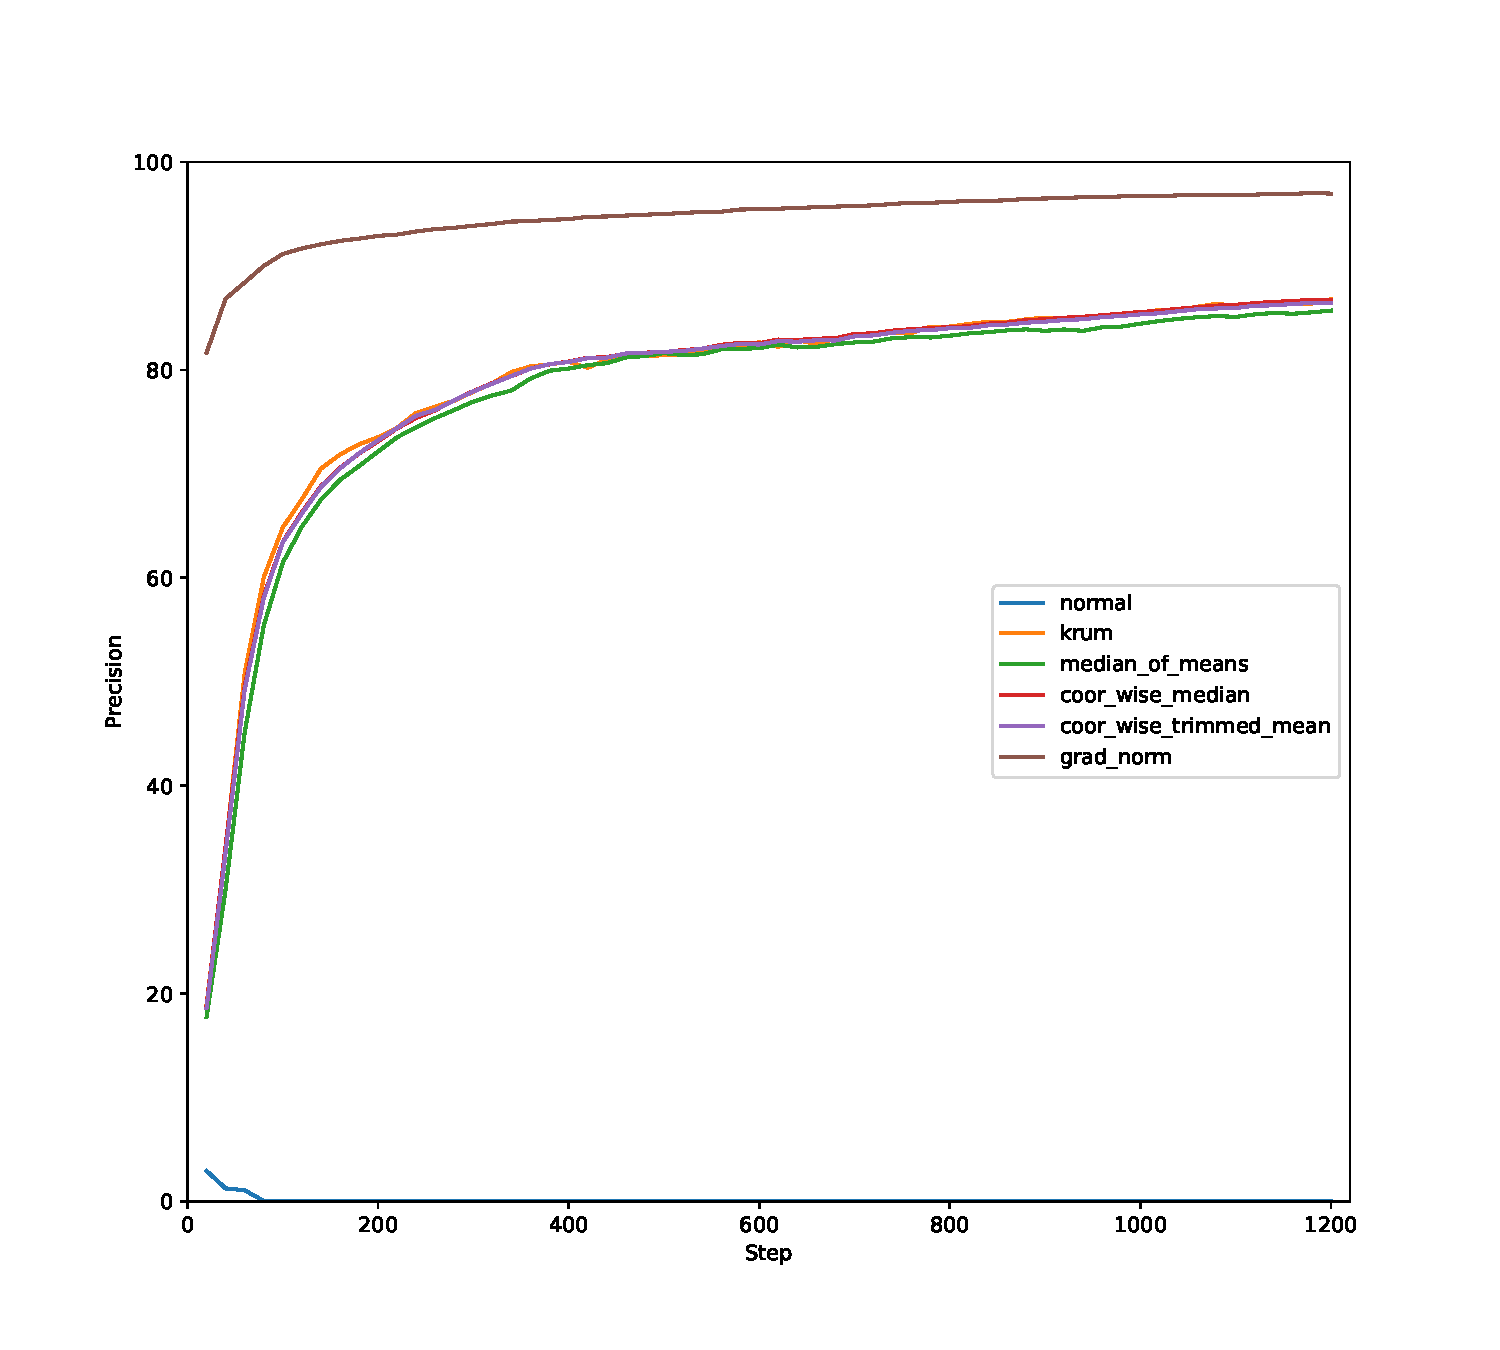
\includegraphics[width=.8\textwidth]{prec1.pdf}
	\caption{Precision@1}
\end{figure}

\begin{figure}
	\centering
	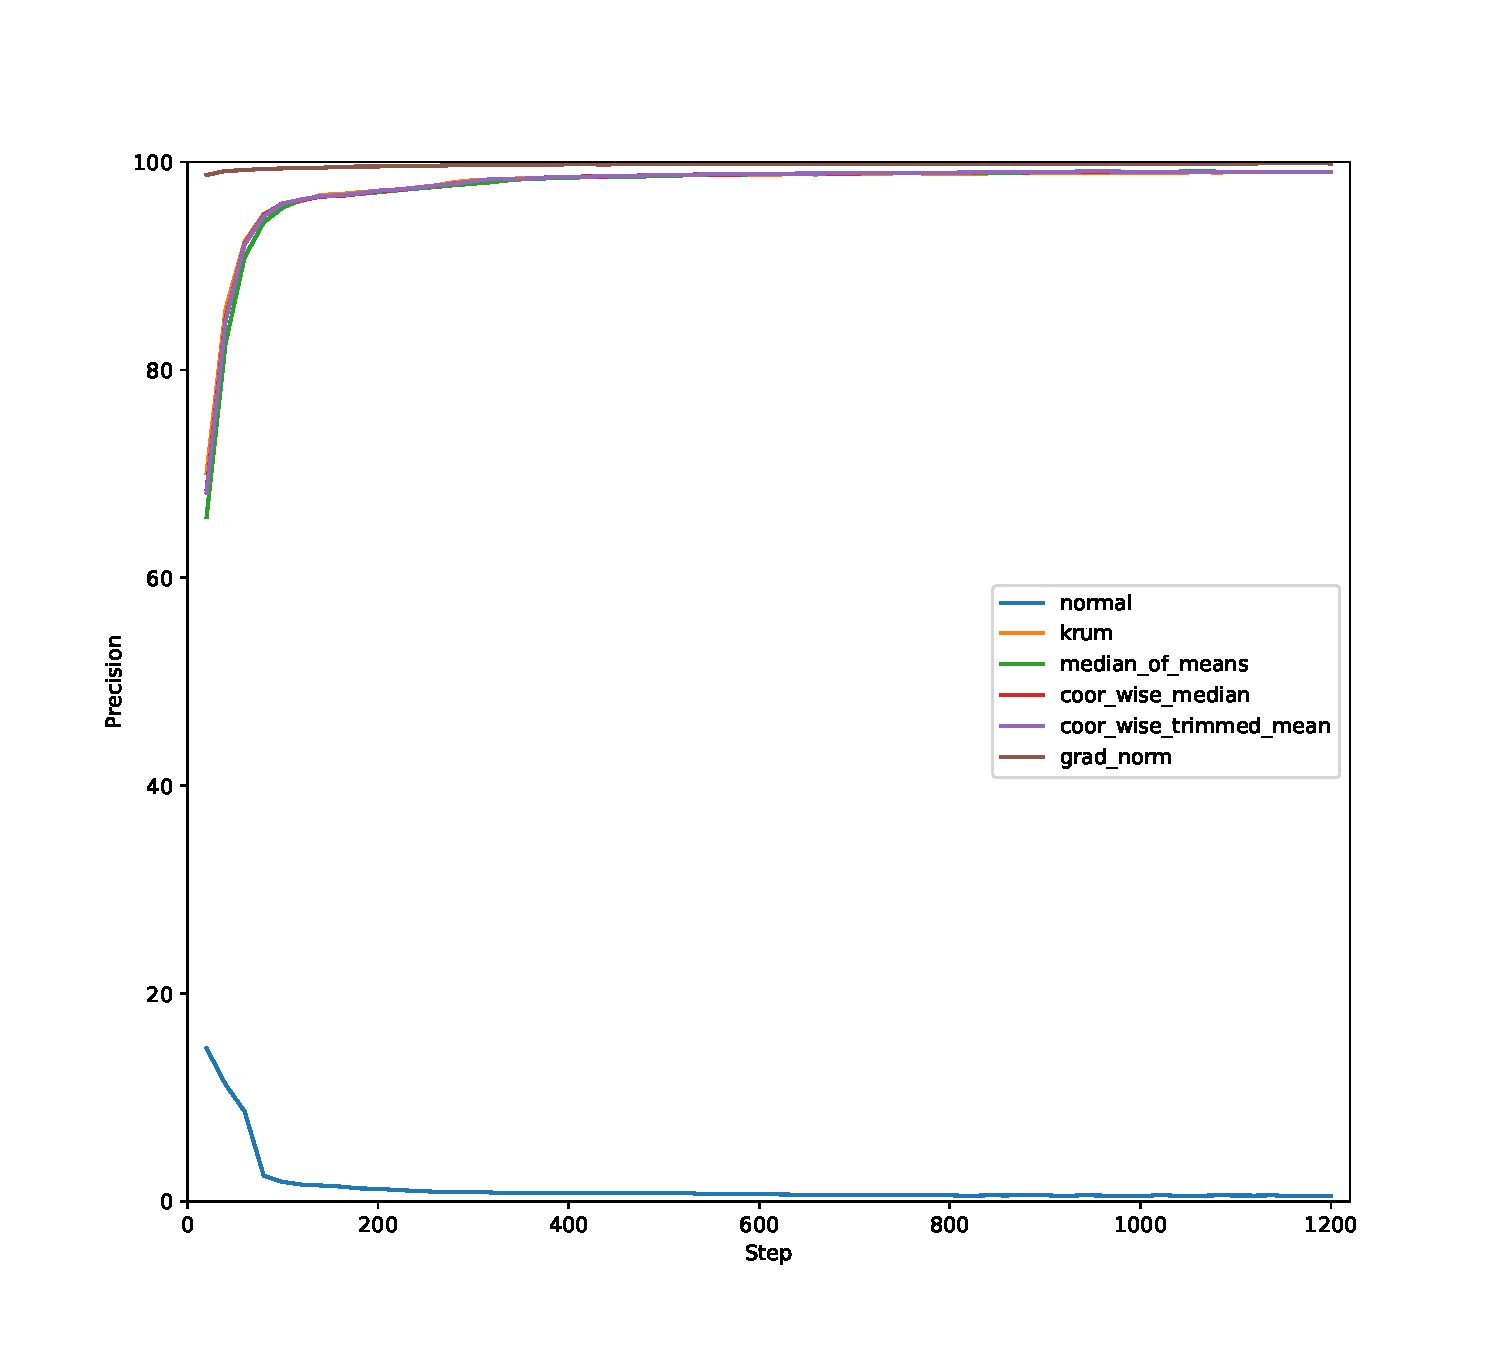
\includegraphics[width=.8\textwidth]{prec5.pdf}
	\caption{Precision@5}
\end{figure}

\end{document}